\subsection{Robustness}\label{subsec:robustness}
The study of robustness concerns the stability of statistical estimation procedure under the existence of outliers.
This has an economical meaning to our hedging exercise: Do we want the optimal hedge ratio react to extreme market changes?
In practice, outliers of returns can come from anywhere, for example, a tweet from Elon Musk, a sudden large order from
institutional investor, or an incident of system failure in cryptocurrency exchanges.
Rapid and drastic changes in portfolio weight causes problem of slippage and transaction cost.
Investors should be aware of the cost brought by the sensitivity of the optimal hedge ratio procedure.
\medskip

The discussion of sensitivity or robustness dates back to \citet{huber1981robust}'s work on robust statistics.
\citet{hampel2011robust} suggest an infinitesimal approach to investigate sensitivity of statistical procedures.
There are three central concepts in this approach, qualitative robustness, influence function, and break-down point.
They are loosely related to the concept of continuity, first derivative of functional, and the distance of a functional to its nearest pole (singularity).
While the first concept is a qualitative feature of a functional, the second the third concepts are practical tools to measure sensitivity quantitatively.
We deploy a finite sample version of the second and third concepts.
Details of robustness of risk measures can be found in \citet{cont2010robustness}. \medskip

\francis{\em [FL: Need to rewrite the following to show the IF of hedge performance instead of h. But Please have a look of the methodology first.]}
With a probability space $(\Omega, \F, \p)$,
we denote $M: \Omega \mapsto \mathscr{C}, M \in \{\text{MLE}, \text{MM}, \text{Empirical}\}$ be estimators of interest for distribution of returns,
$\mathscr{C} = \{\text{Gaussian-Copula}, ..., \text{Plackett-Copula}, \text{Empirical-Copula}\} \in \p$ be a set of bivariate distributions of interest,
$\rho_{h}: \mathscr{C} \mapsto \mathbb{R}$ be a risk measure on the hedged portfolio given $h$,
and finally, $\hat h_\rho = \argmin_h \rho_{h} \circ M$ be a functional to obtain the optimal hedge ratio (OHR) depending on risk measure
$\rho$. \medskip

The influence function of $\hat h_\rho$ with finite sample size $n$ is
\begin{align}
    \text{IF}(\bm{z}; \hat h_\rho) = \frac{\hat h_\rho(\bm{X}_1,...,\bm{X}_n, \bm{z})-
    \hat h_\rho(\bm{X}_1,...,\bm{X}_n)}{\frac{1}{n+1}}.
    \end{align}

\francis{\em [The inclusion of $\bm{z}$ has nothing to do with the probability in a probability space, i.e. it is possible to include points with density zero.]}

The equation describes the effect of a single contamination at point $\bm{z}$ on the estimate of OHR,
standardised by the mass of the contamination. \medskip

Figure~\ref{fig:IFs} shows the influence function of $\hat h_\rho$ of using $t$ copula estimated by MLE with 300 data points of
Bitcoin and CME future returns from 14/12/2018 to 25/02/2020.
Contamination are $[-0.3,-0.27,..., 0.3] \bigotimes [-0.3,-0.27,..., 0.3]$, in total $900$ pairs of contamination. \medskip

We can see from the plots that Expected Shortfall with $\alpha = 99\%$ is very sensitive the negative return in spot (lower right plot).
The $h^*$ obtained this way increases with a single contamination of negative jump in spot price.
VaR at $99\%$ is also sensitive to negative jump in spot price but with a lower level (lower left plot).
This is a natural result that reflect investor's risk strong preference of avoidance: investor increase her future's short position
to compensate potential large drop in spot price.
The result of ES being more sensitive to VaR as risk measure agrees with the conclusion of \citet{cont2010robustness}. \medskip

Other risk measures are relatively less sensitive.
Interestingly, although ERM place heavy weights to negative returns,
its IF is similar to that of variance, where variance does not exhibit risk preference.
\francis{[FL:This might due to the smooth $\phi(p)$ over the spectrum $[0,1]$ of ERM. The $\phi(p)$ of VaR is a Dirac function at a single point $\alpha$, that of ES
has a sharp cut off at $1-\alpha$, a tiny change in rank of $r^h$ causes VaR and ES to shift their weights.]}

\begin{figure}[h!t]
      \centering
   \begin{tabular}[width=20cm, height=20cm]{ccc}
             \centering
   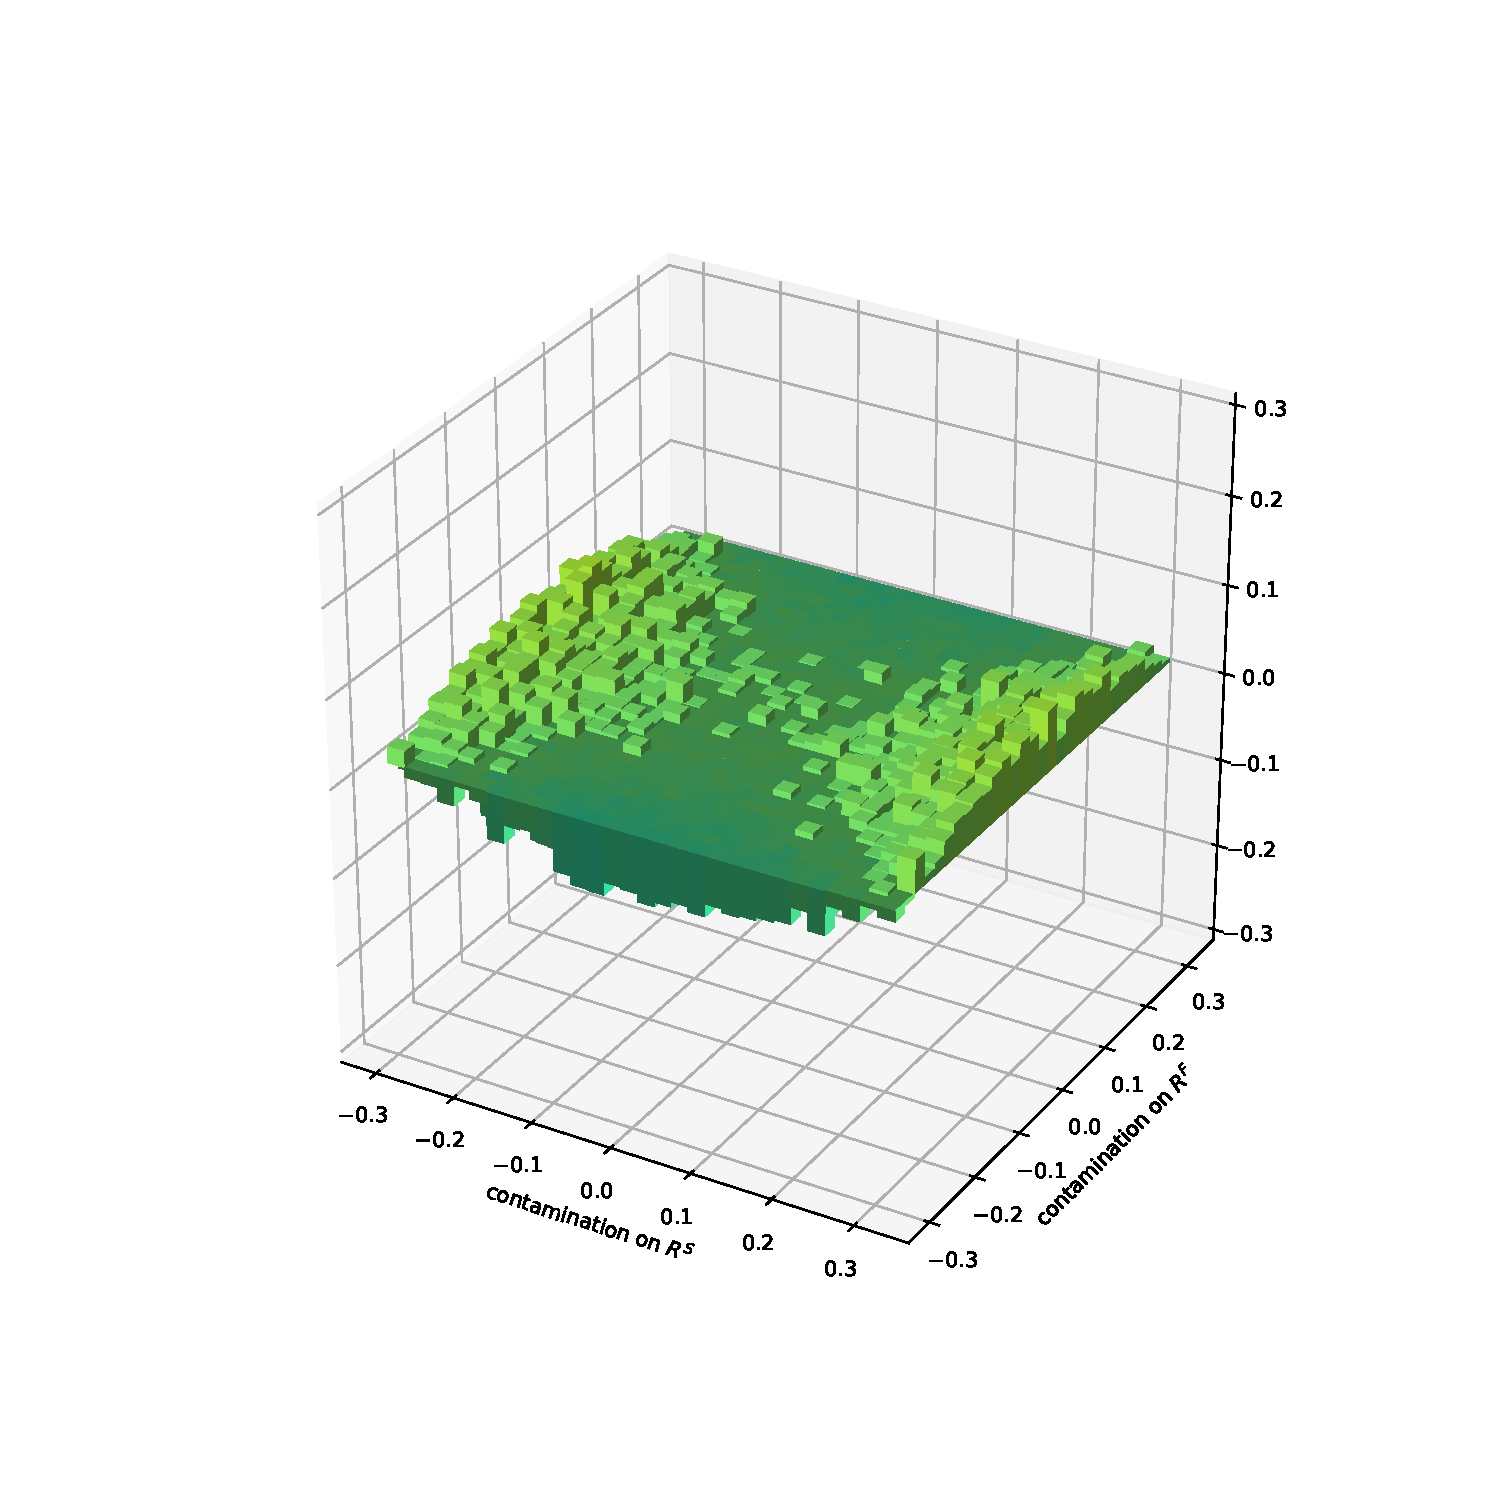
\includegraphics[height=5cm]{_pics/IF_plots/Variance_t_copula_MLE.pdf} &
   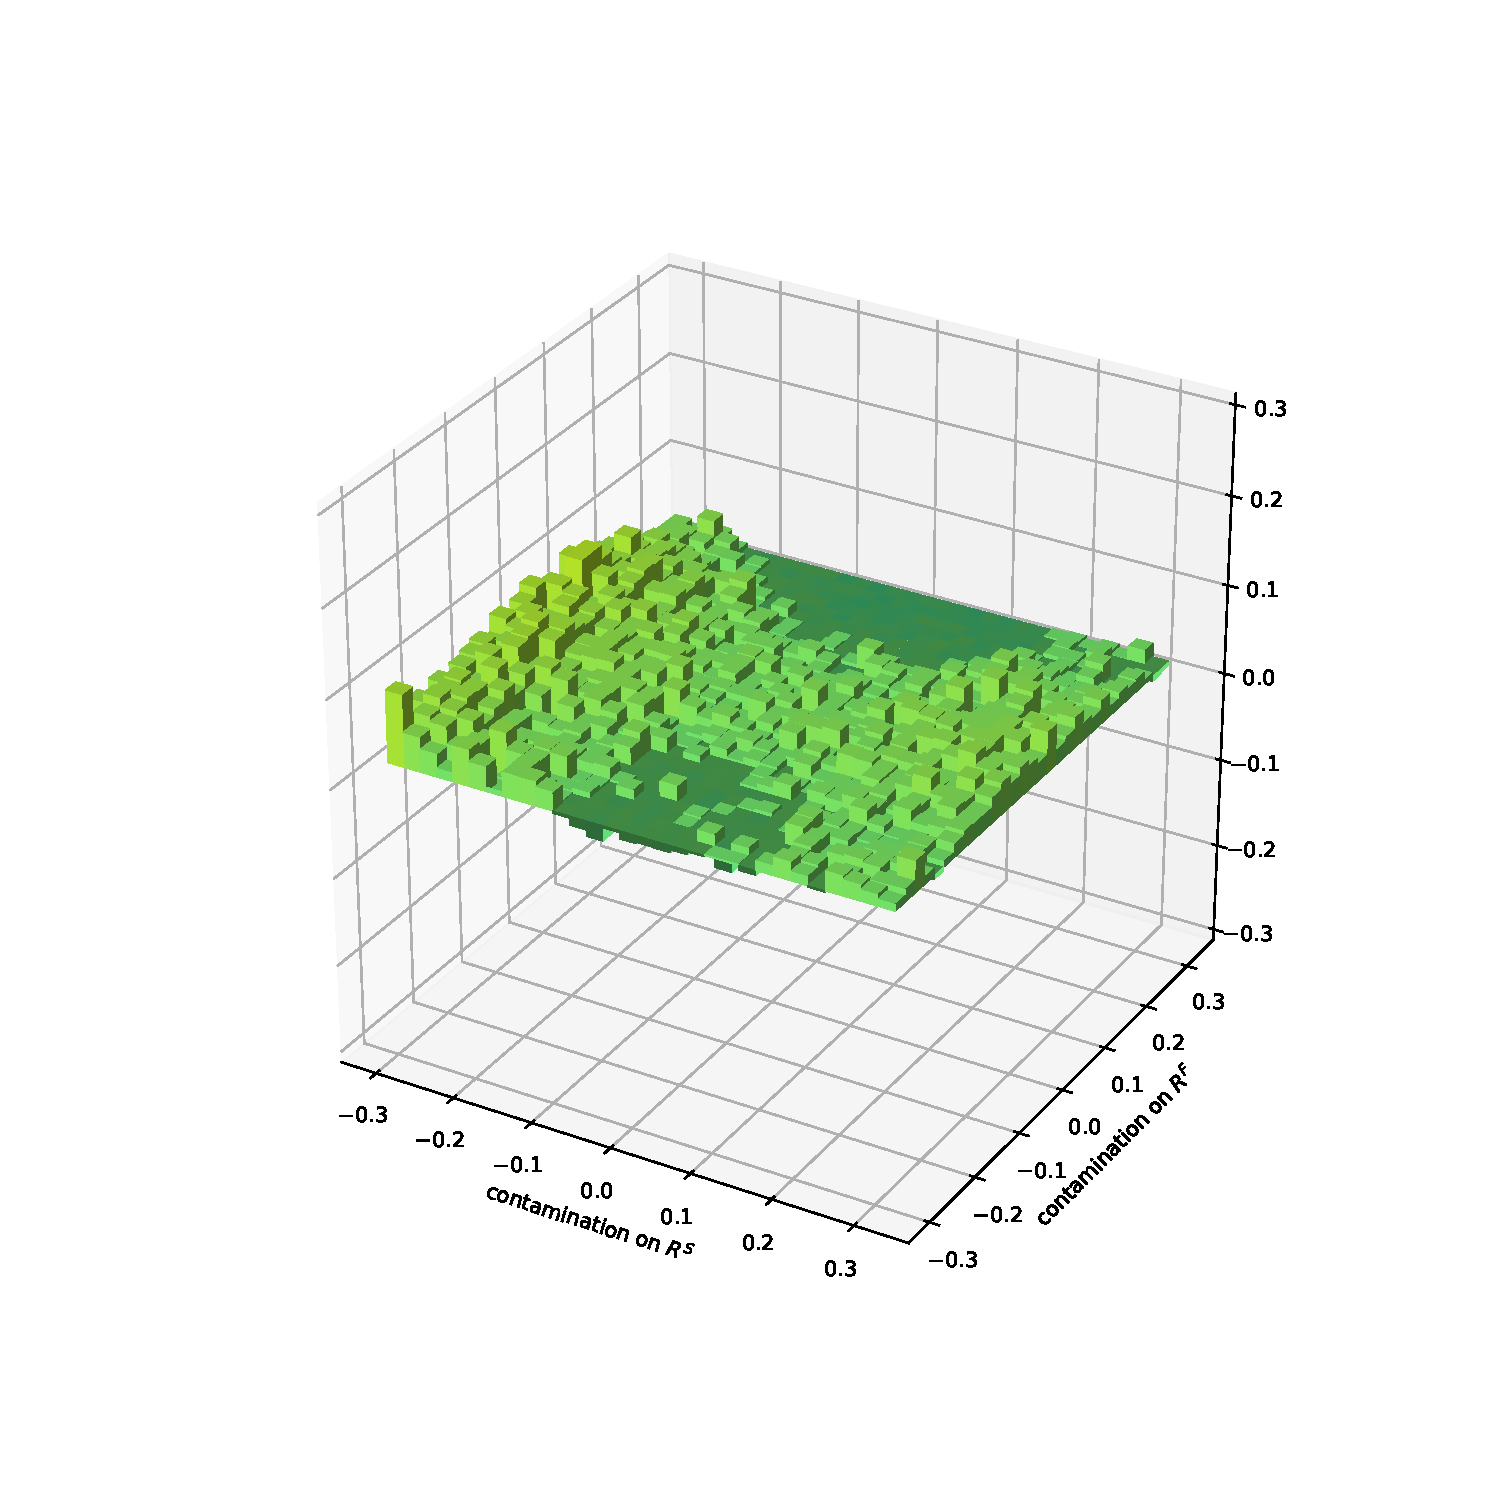
\includegraphics[height=5cm]{_pics/IF_plots/ERM10_t_copula_MLE.pdf}&
   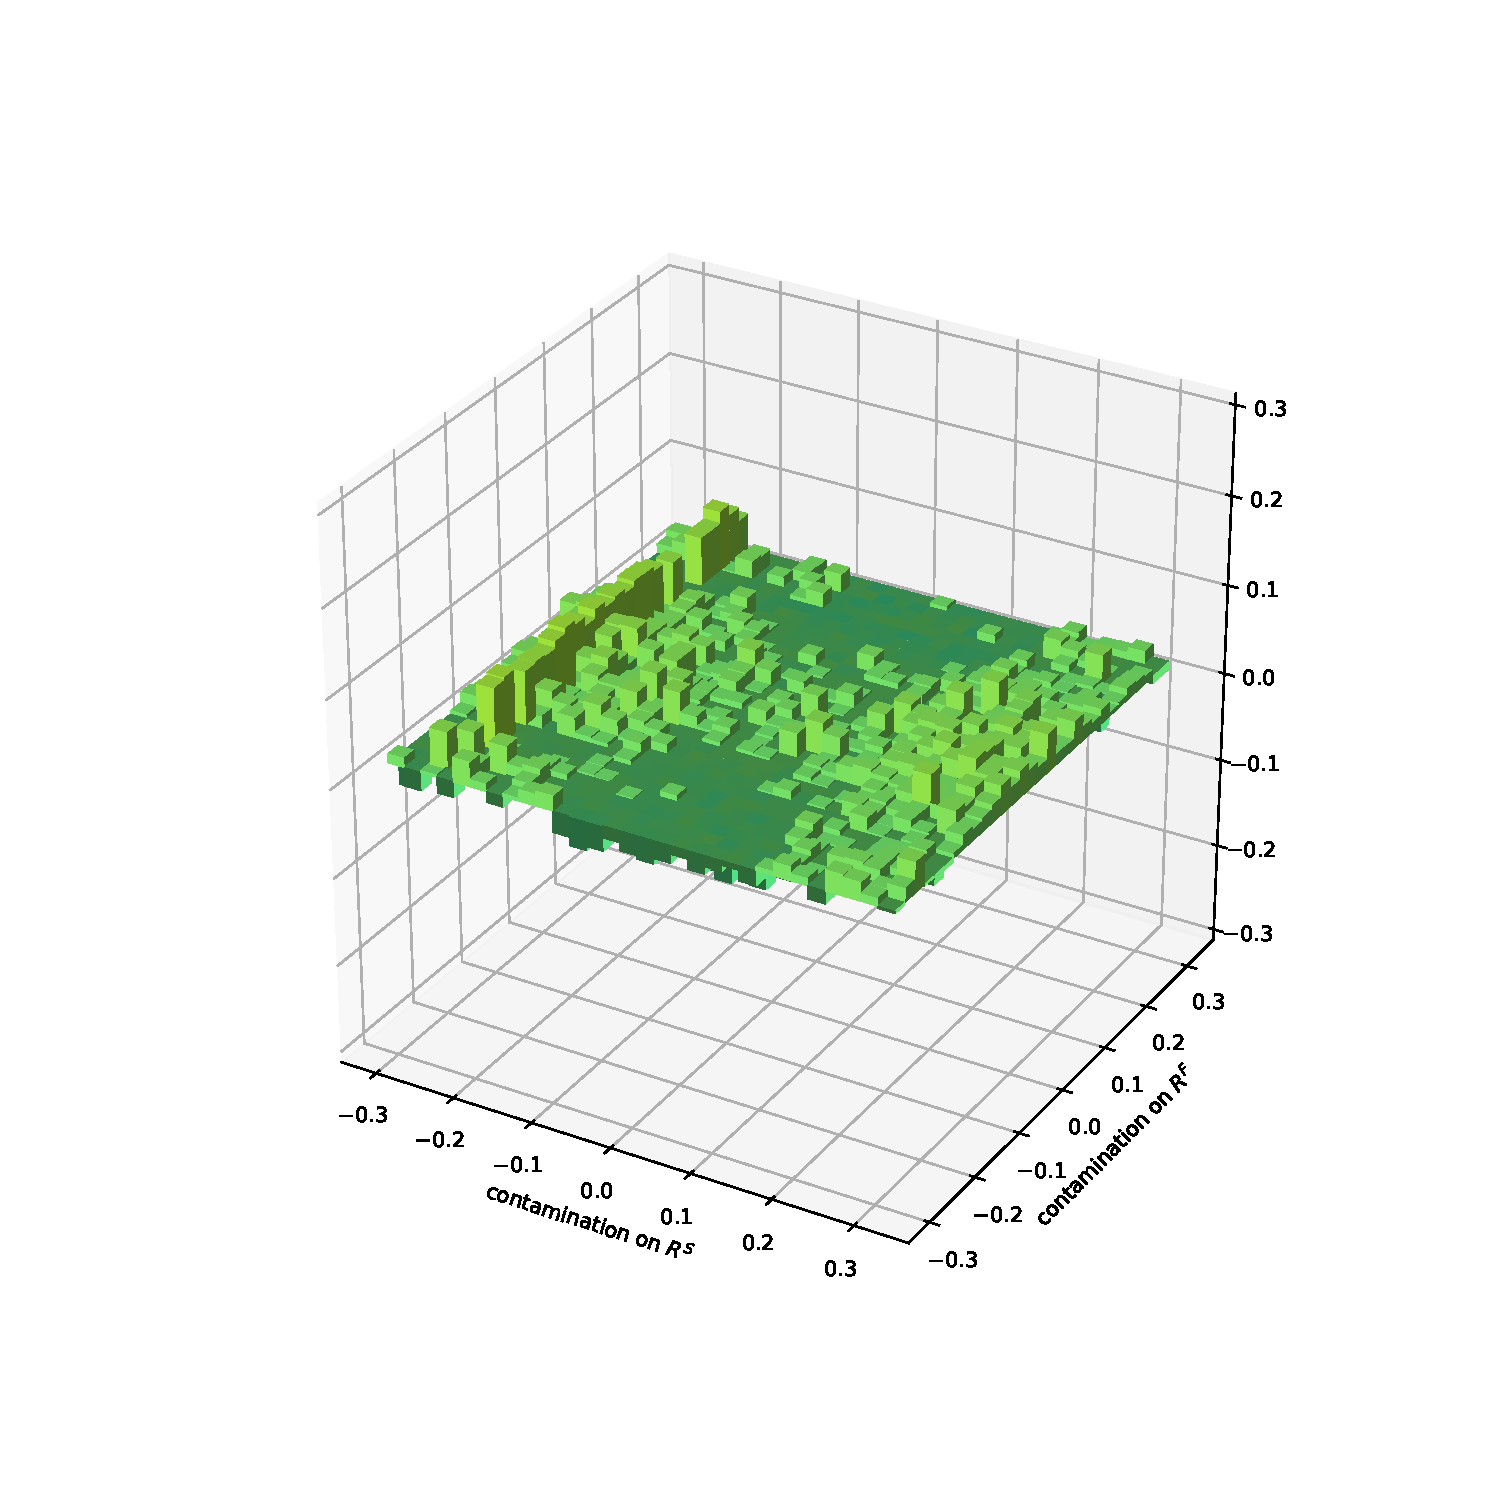
\includegraphics[height=5cm]{_pics/IF_plots/VaR5_t_copula_MLE.pdf} \\
   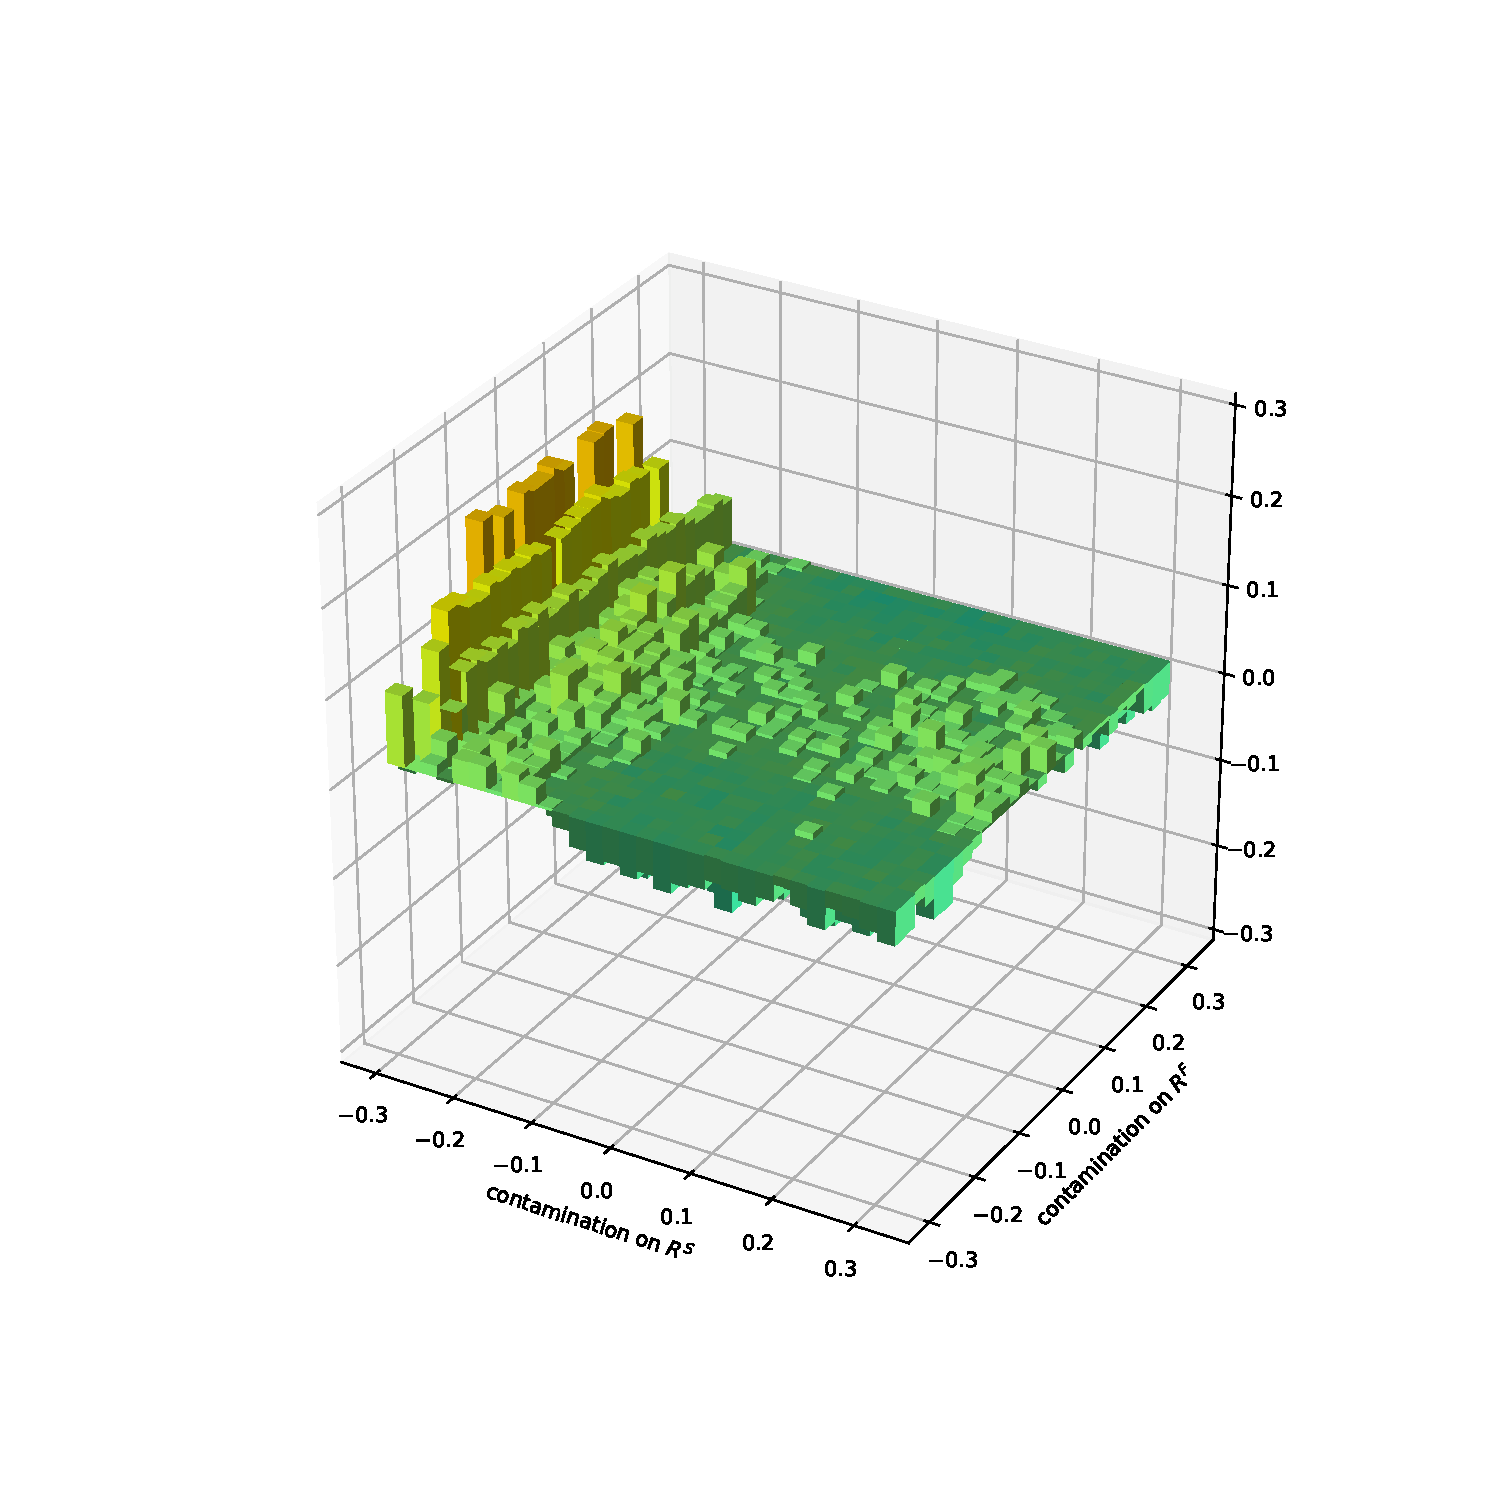
\includegraphics[height=5cm]{_pics/IF_plots/VaR1_t_copula_MLE.pdf} &
   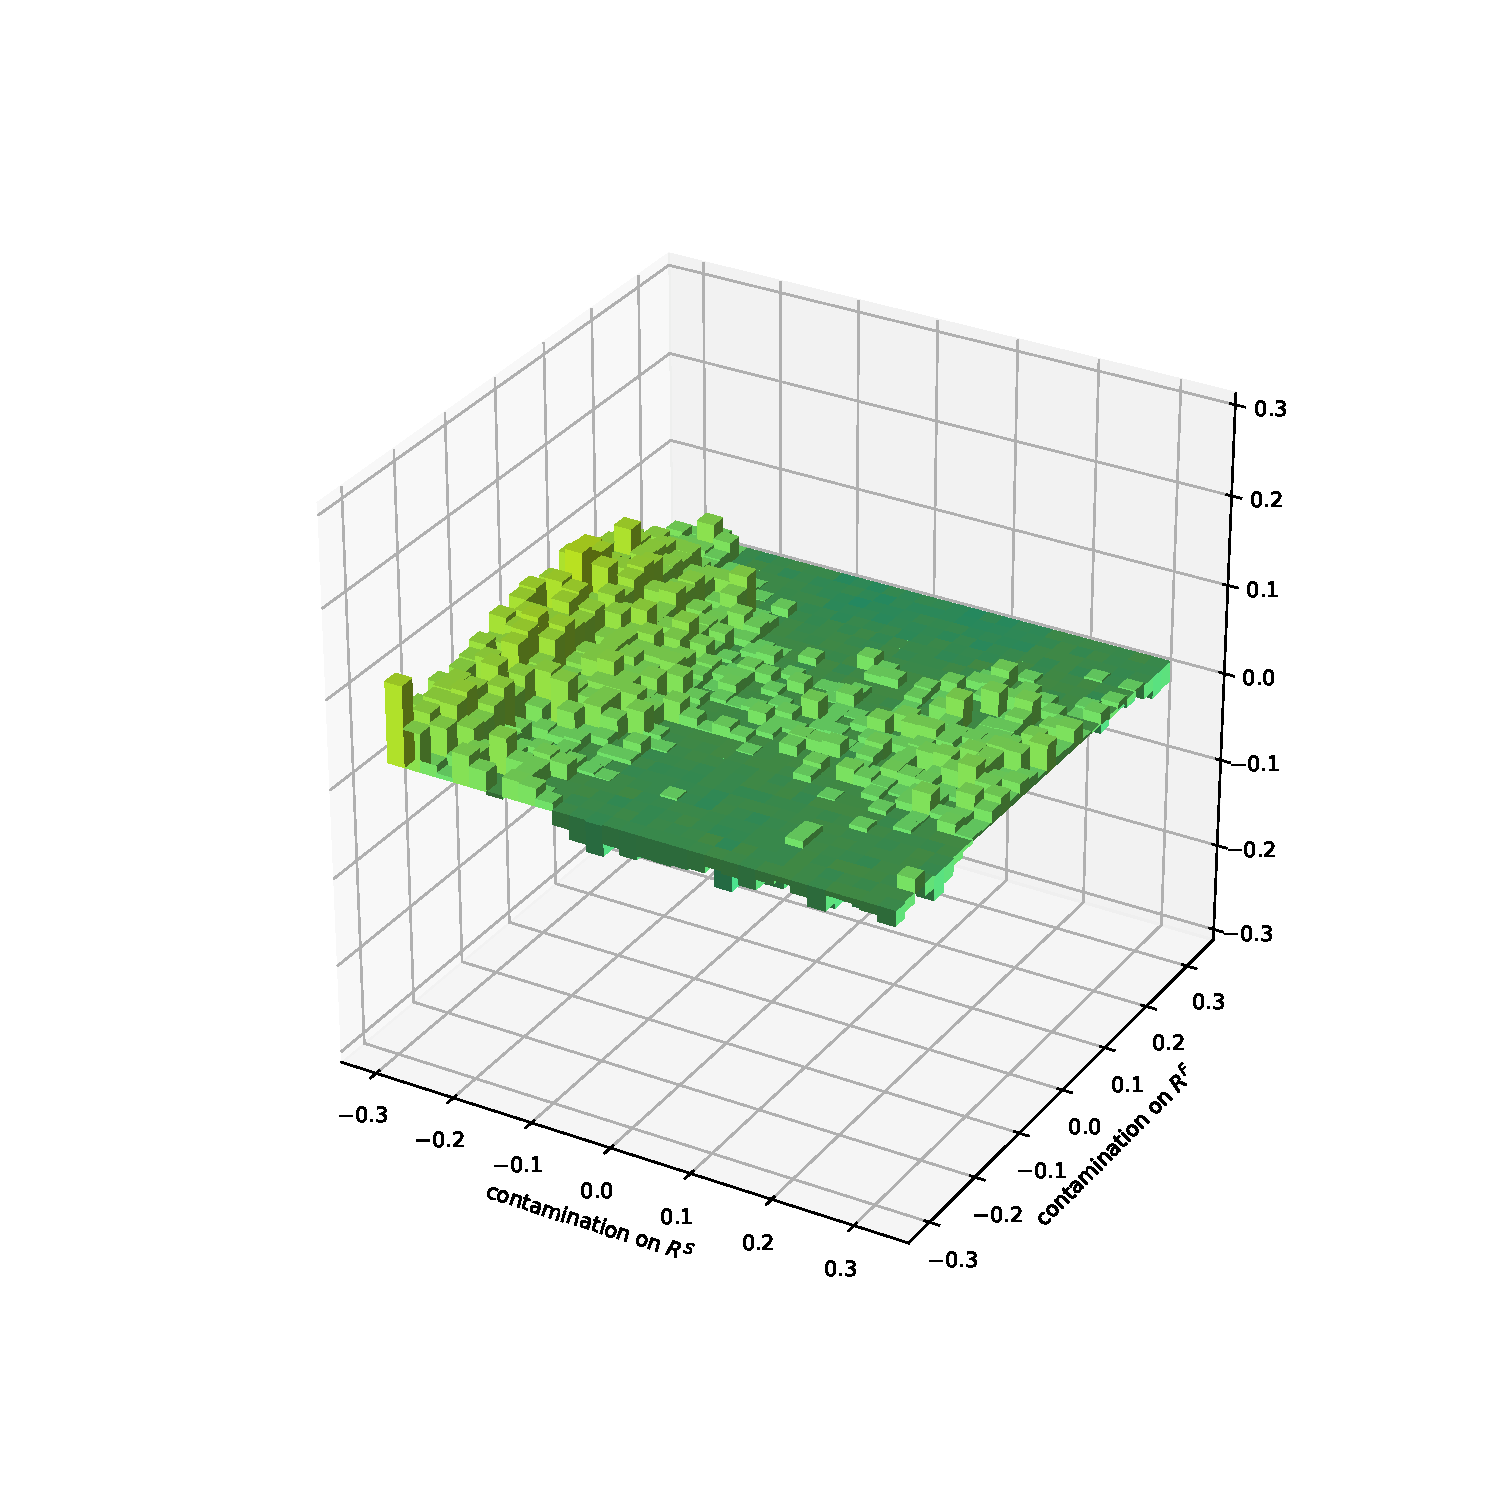
\includegraphics[height=5cm]{_pics/IF_plots/ES5_t_copula_MLE.pdf} &
   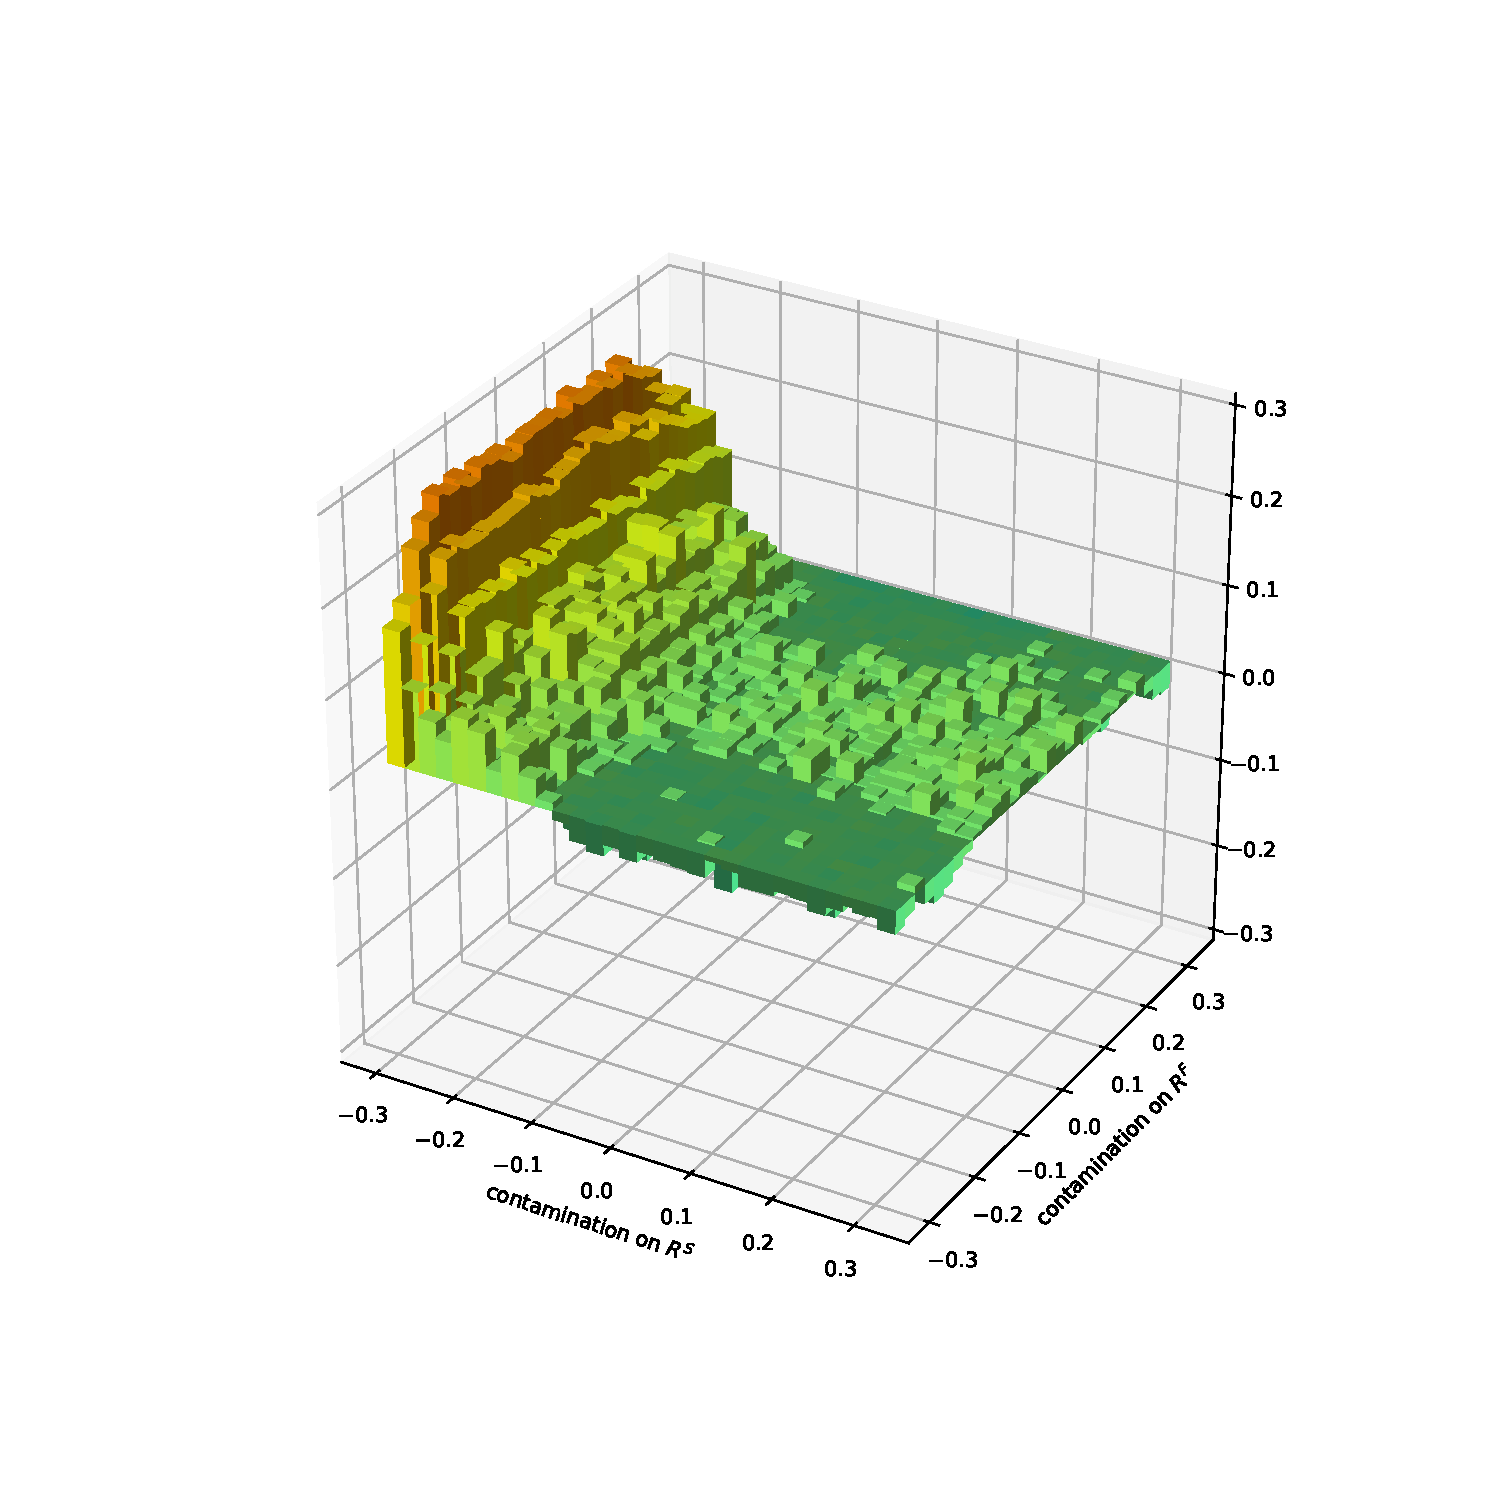
\includegraphics[height=5cm]{_pics/IF_plots/ES1_t_copula_MLE.pdf}
   \end{tabular}
   \caption{Influence functions (IF) of $h^*$ using $t$ copula copula estimated by MLE. From left to right, top to bottem, the plots are
   IF of using $\text{Var}$, $\text{ERM}_{10}$, $\text{VaR}_{0.95}$, $\text{VaR}_{0.99}$, $\text{ES}_{0.95}$, and $\text{ES}_{0.99}$ respectively.
   \href{http://www.quantlet.com/}{
\includegraphics[width=20pt]{_pics/qletlogo_tr.png}}}
   \label{fig:IFs}
\end{figure}